\chapter{Automated Segmentation of Kidneys using Machine Learning}
\label{chap:ML}

\begin{abstract}
	
	
	This work was presented as an aural presentation at the \ac{ISMRM} 28th Annual Meeting (2020) \cite{daniel_automated_2020}.
	
	\lipsum[1]
\end{abstract}
\newpage

\section{Introduction}

Segmentation of the kidneys from \ac{MRI} is a time consuming aspect of many renal \ac{MRI} studies \cite{cox_multiparametric_2017, cohen_mri_2009, van_den_dool_functional_2005}. \ac{TKV} gives insight into renal function and is therefore used as a measured parameter for a variety of renal pathologies. The use of \ac{TKV} is an active area of ongoing research for \ac{ADPKD}, which is characterised by an increase in \ac{TKV} due to cyst formation. Disease progression can be monitored by recording \ac{TKV}, with higher rates of \ac{TKV} increase being associated with a more rapid decrease in renal function \cite{chapman_kidney_2012, tangri_total_2017, grantham_volume_2006}. Measurements of \ac{TKV} in \ac{CKD} subjects have shown a significant correlation with glomerular filtration rate \cite{buchanan_quantitative_2019}, the primary measure of \ac{CKD} severity \cite{stevens_assessing_2006}, with more generally a decrease in \ac{TKV} associated with a decrease in renal function \cite{gong_relationship_2012}. When studying pathologies which commonly lead to a change in kidney function, total kidney perfusion is often measured, this metric relies on an accurate measurement of renal blood flow and kidney volume of each kidney, and allows investigators to ascertain if the blood flow is preserved as the organ changes in size or if tissue perfusion is impaired. In addition to \ac{TKV} measurements, renal segmentation is an important first step for many other processing pipelines, be that for automated cortical-medullary segmentations or to carry out multiparametric mapping within only the kidney to reduce computation times. 

The gold standards of kidney segmentation are manual \ac{ROI} boundary tracing \cite{di_leo_measurement_2011} or stereology \cite{bae_volumetric_2000} by experienced and skilled experts, with blood vessels in the kidney and the hilum excluded. These manual processes are highly time consuming (taking approximately 15 – 30 minutes per subject \cite{zollner_assessment_2012, sharma_kidney_2017, simms_rapid_2019} and can be biased by investigator judgement due to the similar signal intensities between the kidneys and surrounding organs, anatomical differences between subjects, cysts and image artefacts. Consequently, the resulting kidney \ac{ROI}s produced are subject to intra- and inter-expert variability as a result of the varying expertise levels; experts may segment a specific image differently when performed more than once, or different experts may segment the same image differently. These factors mean that the development of a faster and ideally fully automated method of renal segmentation is highly desirable. However the same factors that make manual segmentation difficult can also limit fully automated methods, for example the signal intensity of the kidneys closely matches that of other abdominal structures such as the spleen.

A number of automated methods have been proposed with varied success \cite{zollner_assessment_2012}. Some simply assume the kidney is an ellipse and calculate the volume from measurements of the pole-to-pole distance \cite{cheong_normal_2007, spithoven_estimation_2015} or include a correction factor to reduce overestimations \cite{seuss_development_2017}. Unfortunately these techniques produce a large confidence interval and still require human intervention to define the pole-to-pole length, a process that can produce inconsistencies between readers and takes a reasonable amount of time ($\approx$5 min) \cite{magistroni_review_2018}. Other semi-automated methods use classical image processing techniques such as thresholding \cite{coulam_measurement_2002}, water-shedding \cite{karstoft_different_2007}, level sets \cite{simms_rapid_2019, gloger_prior_2012}, and spatial prior probability mapping \cite{kim_automated_2016}. These methods can either be inaccurate, over-segmenting the kidneys, or include a number of parameters that need to be manually adjusted and are computationally intensive. Further, the fact that each technique is highly optimised for a specific dataset means that it needs to be re-written to be applied to different pathology, another time consuming and highly skilled process.

Machine learning methods have the potential to automatically detect different patterns from data given to a model which has been trained. Deep learning is a class of machine learning algorithms that can model high-level information in an image using several processing layers of transformations. This uses an architecture of multi-level linear and non-linear operations, described by layers, to learn complex functions that can represent high-level detail to map the input data to the output segmentations directly. As more data becomes available the algorithm can become more accurate and generalised, without a need to rewrite the underlying methods, thus making it a good choice for long term development. 

In recent years, deep learning-based methods have been applied to the segmentation of medical images, especially successful has been the U-Net \cite{ronneberger_u-net_2015}. This modified fully \ac{CNN} architecture uses a number of convolution, pooling and up-sampling layers to detect features in the input data at multiple resolutions. The convolution layers convolve a learnable kernel with the input data to generate spatial feature maps that are passed to subsequent layers in the network. By adjusting the kernels, the resulting feature maps can be optimised to detect the location of the kidneys. Pooling layers are used to down-sample the data and allow some convolution kernels to become tuned to approximate features, this also reduces the tendency of the network to overfit the training data. When the data has been fully down-sampled, up-sampling layers are used to increase the resolution of the feature maps back to that of the original data while more convolution layers also learn the precise location of the kidneys. Parameters are adjusted by comparing the output from the network to a known ground truth. \ac{CNN} methods have been applied to segmentation in other areas of medical imaging \cite{lu_automatic_2017, sharma_automatic_2017, wachinger_deepnat_2018, fu_novel_2018}, for example to prostate segmentation of \ac{MRI} images \cite{hassanzadeh_convolutional_2019}, liver segmentation of x-ray \ac{CT} images \cite{li_h-denseunet_2018} and segmentation of polycystic kidneys \cite{kline_performance_2017, van_gastel_automatic_2019, shin_expert-level_2020}. However, to date, these methods have not been successfully applied to \ac{CKD} and healthy kidney segmentation from MR images. 

Here a single 2D U-Net model \ac{CNN} is used for the segmentation of the kidneys in both \ac{HC} participants and \ac{CKD} patients using \ttwo-weighted MR images. Automatically generated kidney masks are compared with manual masks defined by experts and assessed for similarity using multiple voxel and surface based metrics and total segmented volume. A subset of subjects were scanned multiple times to assess the repeatability of the segmentations.

\newpage
\section{Methods}
The study was approved by the University of Nottingham Medical School Research Ethics Committee (H14082014 and E14032013), and East Midlands Research Ethics committee REC reference: 17/LO/2036 and 15/EM/0274.

\subsection{MRI Data Acquisition}
\label{sec:ml_methods_acquisition}

All kidney \ac{MRI} scans were acquired on a 3T Philips Ingenia system (Philips Medical Systems, Best, The Netherlands) using a 2D \ttwo-weighted \ac{HASTE} sequence optimised to achieve the maximum contrast between the kidneys and surrounding tissue (\ac{TE} = 60 ms, \ac{TR} = 1300 – 1800 ms, \ac{SENSE} factor = 2.5, refocus angle 120$\degree$, bandwidth, 792 Hz, \ac{FOV} = 350 x 350 mm$^2$, voxel size = 1.5 x 1.5 x 5 mm$^3$ and a slice gap of 0.5 mm with approximately 13 coronal slices, enough to image the entire kidney \cite{petzold_building_2014, will_automated_2014}, in a single 17 - 23 s breath hold.

The dataset consisted of 60 subjects, 30 \ac{HC} (10 female, 20 male) with a mean age of 26 $\pm$ 11 (19–77) years and 30 \ac{CKD} patients (6 female, 24 male) with a mean age of 59 $\pm$ 14 (19–80) years and mean \ac{CKD} Stage 3.5 $\pm$ 1.2 (1-5). Ten of the subjects (5 \ac{HC}s and 5 \ac{CKD} patients) were scanned five times in the same scan session for use as test data. In each test data scan session, subjects were repositioned between each acquisition (removed from the scanner, asked to sit up and move on the bed), additionally the scanner operator attempted to vary the acquisition geometry between each scan while still acquiring full kidney coverage. These repeated test datasets allow the consistency of the networks ability to measure \ac{TKV} to be assessed. 

In total, 649 2D image slices from the 50 subjects in the training data and 650 2D image slices from the 10 subjects in the test data, were collected. A summary of the data collected is provided in Table \ref{tab:ml_datasets} and Figure \ref{fig:ml_true_tkv_hist}.

\begin{table}[h]
	\centering
	\begin{tabularx}{\textwidth}{X|XXXXXX}
		\hline
		& \textbf{Number of Subjects} & \textbf{Number of Datasets} & \textbf{Number of 2D Slices} & \textbf{Sex (F/M)} & \textbf{Mean Age} & \textbf{TKV (m$\ell$)} \\ \hline
		\textbf{Training HC}  & 25                          & 25                          & 325                          & 9/16               & 26 $\pm$ 12       & 296 $\pm$ 38           \\
		\textbf{Training CKD} & 25                          & 25                          & 324                          & 6/19               & 58 $\pm$ 15       & 258 $\pm$ 72           \\
		\textbf{Testing HC}   & 5                           & 25                          & 325                          & 1/4                & 25 $\pm$ 3        & 330 $\pm$ 35           \\
		\textbf{Training CKD} & 5                           & 25                          & 325                          & 0/5                & 69 $\pm$ 3        & 274 $\pm$ 56          
	\end{tabularx}
	\caption{Characteristics of datasets used for training and validation of the 2D U-Net model \ac{CNN}.}
	\label{tab:ml_datasets}
\end{table}
\todo{Fix table \ref{tab:ml_datasets} formatting}
\begin{figure}[h]
	\centering
	\includegraphics[width=0.7\textwidth]{ML/Datasets/dataset_hist_overlay.pdf}
	\caption{Distribution of \ac{TKV} within the training and testing data.}
	\label{fig:ml_true_tkv_hist}	
\end{figure}

\subsection{Manual Segmentation}
The manual binary mask of the kidneys of each subject were generated by one of three observers (A, B and C who had been trained on kidney segmentation and had an average of 2 years of experience), with each observer segmenting data from both the training and testing datasets. Kidney boundaries were manually traced using freely available software (MRIcron \cite{rorden_neurolabuscmricron_2021}) and any area of non-renal parenchyma, such as the renal hilum and cysts, were excluded from the manual definition. Binary masks of the kidney were generated, and the volume of each kidney was computed from the product of the number of voxels in each kidney mask and the voxel volume. Separate kidney volume for the left and right kidneys was determined and summed to compute \ac{TKV}. All measurements were performed by observers blinded for patient number and previous \ac{TKV} measurements. 

For the training phase, for each subject a manual mask was used from a single observer (randomised between observer A, B, or C). For the testing phase, all five scans from a given subject were segmented by a single reader with the ten subjects being segmented by a mix of the three readers i.e. the test data comprised of subjects segmented by all readers but the repeat scans of each subject were segmented by the same reader. For four \ac{HC} subjects from the test dataset, manual masks were drawn by all three observers for all five repeat acquisitions to allow assessment of inter-observer variability in the manual masks. \ac{HC}s were chosen for this analysis as they healthy kidneys have a more consistent morphology and thus will give a best-case measure of observer variability and provide a comparison of the automated method to the highest standard of manual segmentation.

\subsection{Automated Segmentation Using a CNN Architecture}

Voxel intensities were normalised between 0 and 255, where 0 was set to the mean voxel intensity minus 0.5 times the standard deviation of that slice and 255 was set to the mean voxel intensity plus four times the standard deviation of the volume. This empirically derived windowing led to a clear contrast between the kidneys and surrounding tissue while negating the effects of bulk signal changes between volumes. Each dataset volume was then split into 2D coronal slices and resampled to a matrix size of 256 $\times$ 256. Twenty percent of slices were reserved for validation during the network optimisation process, this validation data was used to monitor over-fitting and direct the optimisation process between epochs. Once the data had been split into training and validation sets, the slice order was randomised within sets. Splitting the data before slice randomisation limited the possibility of slices from only one  subject being split over both the training and validation datasets. During training, data augmentation was applied. At the start of each epoch, a batch of images and their corresponding masks was selected at random from the training data and a series of random shifts (up to 25 \% of the image in both the horizontal and vertical direction), zooms (between 0.75 and 1.25 magnification), rotations (within a 20$\degree$ range), and sheers (within a 5$\degree$ range) were applied to the image/mask pair to produce different yet anatomically reasonable images. The weights of the network were then adjusted based on this augmented data before selecting a new batch of images for the next epoch. Augmenting the data reduces the tendency of a model to over-fit the training data and thus increases accuracy when the model is applied to unseen images. 

The U-Net consists of two Fully Convolutional Neural Network-like structures that are cascaded in the form of an encoder-decoder (autoencoder) structure. The encoder is used for feature extraction and the decoder is used for feature mapping to the original input resolution. A summary of the network architecture is shown in Figure \ref{fig:ml_network}. The convolution layers use a set of small parameterised filters, referred to as kernels, to perform convolution operations to produce different feature maps of their input. Here each convolution and deconvolution layer uses a 3 x 3 kernel. Activation layers use a \ac{ReLU}. Following convolution at each resolution, max pooling with a stride 2 is used on the encoding half of the network.

\begin{figure}[h]
	\centering
	\includegraphics[width=1\textwidth]{ML/Model/Model.eps}
	\caption{The architecture of the network used.}
	\label{fig:ml_network}	
\end{figure}

The network was implemented using Keras (v2.2.4) \cite{chollet_keras_2015} with a TensorFlow backend (v1.13.1) \cite{abadi_tensorflow_2015} in Python 3.6.9. All training was carried out on an NVIDIA Titan Xp \ac{GPU} (3840 CUDA cores, 12 GB GDDR5X). The network uses a Dice score loss function, given by,
\begin{equation}
	D\left(A, B\right) = \frac{2\left| A \cap B \right|}{\left|A\right|+\left|B\right|} = \frac{2TP}{2TP + FP + FN},
	\label{eq:dice}
\end{equation} 
where $TP$ is true positive, $FP$ is false positive and $FN$ is false negative. A value of 1 implies complete overlap between the automated mask and the manual mask while 0 implies no overlap. This function is ideal for renal segmentation as it does not weight true negatives which represent the majority of voxels input to the network and thus means that while the network is training, it does not become trapped in a local minimum outputting solely background voxels. Training was carried out over 150 epochs using stochastic gradient descent with an initial learning rate of 0.01 and learning rate decay of $5\times10^{-7}$ and momentum of 0.8, these parameters help the optimiser converge quickly while also avoiding overshooting. As seen in Figure \ref{fig:ml_training_history}, after 150 epochs the validation Dice score plateaued while the training Dice score was still rising slightly, indicating that any further training would lead to over-fitting. Training took approximately thirty minutes.

\begin{figure}[h]
	\centering
	\includegraphics[width=0.7\textwidth]{ML/Training_progress/training_history.png}
	\caption{Dice score of the network for the training and validation data. Data is shown with a 10 epoch rolling average.}
	\label{fig:ml_training_history}	
\end{figure}
\todo{Swap this for eps/pdf rather than png}

\subsection{Statistical Analysis}

Baseline demographics are reported as mean $\pm$ \ac{SD}. Inter-observer variability in manual segmentation and \ac{TKV} was calculated by comparing the \ac{TKV} of the manual masks each observer generated for a given volume, and also assessing the Bland-Altman and regression analysis. Intra-observer variability in manual segmentation was calculated by comparing the \ac{TKV} of the five masks generated by an observer for a given subject. For each, the mean \ac{CoV}; defined as standard deviation/mean and \ac{ICC} were used as measures of repeatability of \ac{TKV}. Voxel-based (e.g. Dice score) and surface based (e.g. Hausdorff Distance)\question{Probably need to say what this is} metrics were also calculated between each observer.

The performance of the automated segmentation was assessed using multiple voxel and surface based similarity metrics. Performance was further assessed by determining the mean difference in \ac{TKV} between the automatic and manual methods. Both actual and percentage (\%) difference in \ac{TKV} were evaluated. Bias (mean) obtained from the automatic and manual methods was assessed using a paired sample t-test. The mean \ac{CoV} and \ac{ICC} were also used as measures of repeatability of the automated \ac{TKV}.

\section{Results and Discussion}

Initial data was collected with a \ac{TR} of 1800 ms leading to a breath hold of approximately 23 seconds. Some subjects struggled to hold their breath for this long on expiration, therefore the effects of reducing the \ac{TR} of the sequence were investigated. As can be seen in Figure \ref{fig:ml_tr}, there is no degradation in image quality from the image with \ac{TR} or 1800 ms to that with at \ac{TR} of 1300 ms, the differences between these images are mainly due to the small movements between volumes, as can be seen in the difference data where the largest differences are seen around the periphery of the kidneys and in the gut. Moving forward, the \ac{TR} was reduced to 1300 ms leading to a sequence with a breath hold of approximately 17 seconds.

\begin{figure}[H]
	\centering
	\includegraphics[width=1\textwidth]{ML/TR/TR_Master_V0_1.eps}
	\caption{The effects of changing the \ac{TR} of the sequence.}
	\label{fig:ml_tr}	
\end{figure}

To verify that the trained network is behaving as expected saliency maps were produced, Figure \ref{fig:ml_salency}, this is especially important given the black box nature of machine learning methods. This map shows the areas the network is using most in its classification \cite{mahapatra_visual_2016}. It verifies that the networks is using the outside areas of the kidney to make its prediction with areas of a similar intensity receiving some attention to distinguish them from the kidney. While this is precisely what is expected of the algorithm, it is important to check this as it is possible for such a method to have learnt a slightly different mechanism for the segmentation, one that is more prone to errors if new data is presented to it.

\begin{figure}[H]
	\centering
	\includegraphics[width=.4\textwidth]{ML/Salency/MSE_Salency.png}
	\caption{An example saliency map of the areas the network uses most when segmenting the kidney.}
	\label{fig:ml_salency}	
\end{figure}

To assess the accuracy of the network, each of the five volumes per validation subject was segmented by the trained network, in theory the \ac{TKV} predicted for each volume should have been the same. Figure \ref{fig:ml_validation} shows the predicted \ac{TKV} against the manually segmented ``true" \ac{TKV} with each subject plot in a different colour. While there is a spread in the predicted values, there is also a reasonable variation in manual \ac{TKV}. For three out of the seven repeatability subjects, the predicted \ac{TKV} has a smaller standard deviation than the manually segmented data, this indicates that the algorithm may actually be more consistent than the humans. To identify if a systematic error is present, a Bland-Altman plot was generated (Figure \ref{fig:ml_ba_validation}). From this figure it is possible to see that the algorithm is slightly over estimating the \ac{TKV} by 0.69\% (1.6 mm$^3$) but there is no correlation between difference in \ac{TKV} and true \ac{TKV} over all subjects. There is a more subtle trend between each repeat on the same subject though, the volumes with a smaller true \ac{TKV} are consistently over estimated more than those volumes with a larger true \ac{TKV}. This again points to an issue with the manual segmentation rather than the algorithm.

\begin{figure}[H]
	\centering
	\begin{subfigure}[c]{0.47\textwidth}
		\centering
		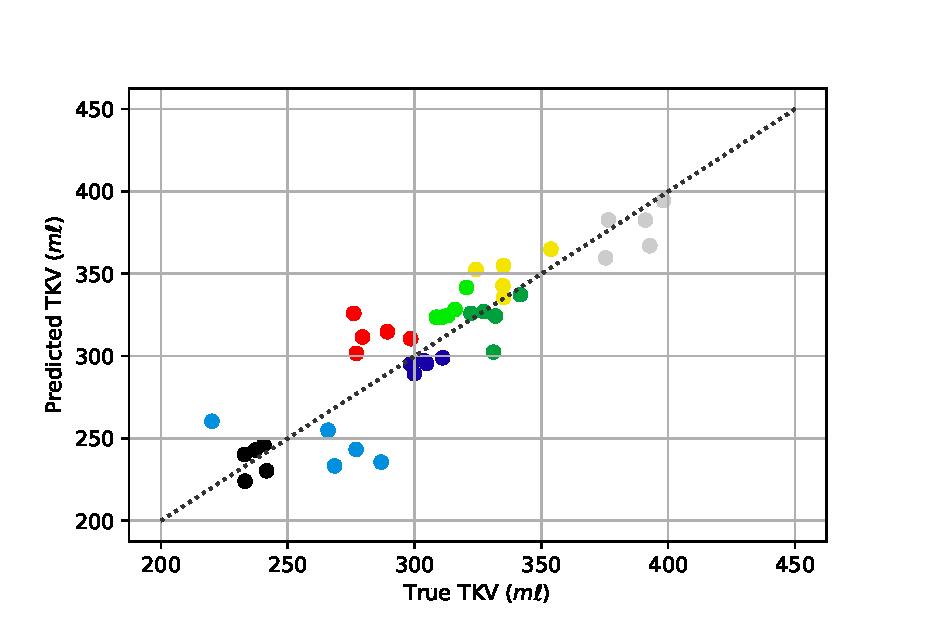
\includegraphics[width=1\textwidth]{ML/BA_plots/190802_training_data_shuffle_input_and_slices_max_dice_09013_validation_tkv.eps}
		\caption{}
		\label{fig:ml_validation}
	\end{subfigure}
	\hfill
	\begin{subfigure}[c]{0.47\textwidth}
		\centering
		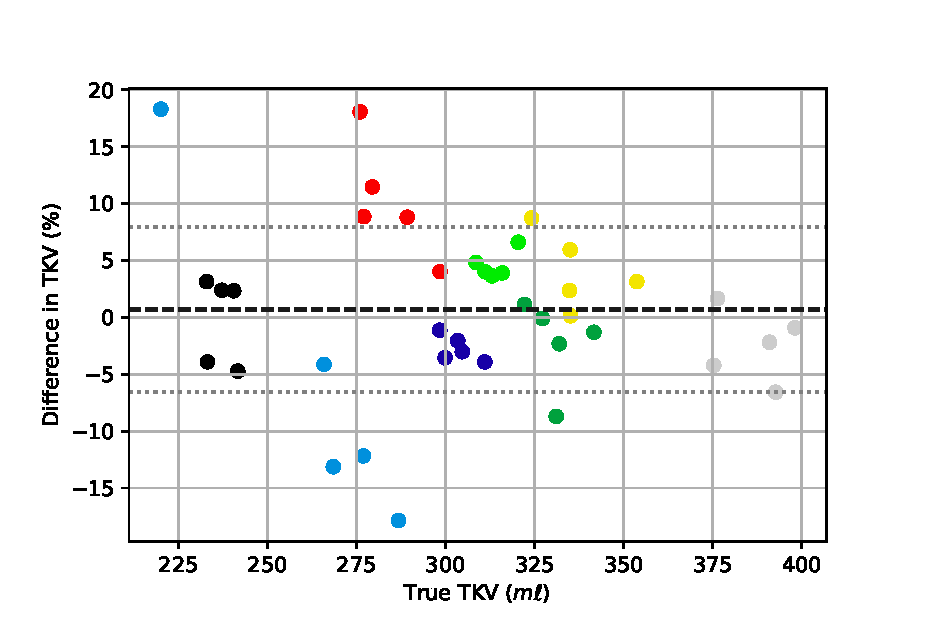
\includegraphics[width=1\textwidth]{ML/BA_plots/190802_training_data_shuffle_input_and_slices_max_dice_09013_validation_ba.eps}
		\caption{}
		\label{fig:ml_ba_validation}
	\end{subfigure}
	\caption{(\subref{fig:ml_validation}) The predicted \ac{TKV} plot against the manually segmented ``true'' \ac{TKV}. Each subject is plot in a different colour. (\subref{fig:ml_ba_validation}) A Bland-Altman plot to identify and systematic error in the networks performance. Each subject is plot in a different colour.}
	\label{fig:ml_validation_tkv}
\end{figure}

While assessing the ability of the algorithm to predict \ac{TKV} is important, it is also necessary to access the raw segmentation as, for example, the algorithm may be over-estimating the size of central slices but under-estimating the size of edge slices. This type of inaccuracy could be masked in the \ac{TKV} however will be visible in the dice scores. These are shown in Figure \ref{fig:ml_validation_dice}.

\begin{figure}[H]
	\centering
	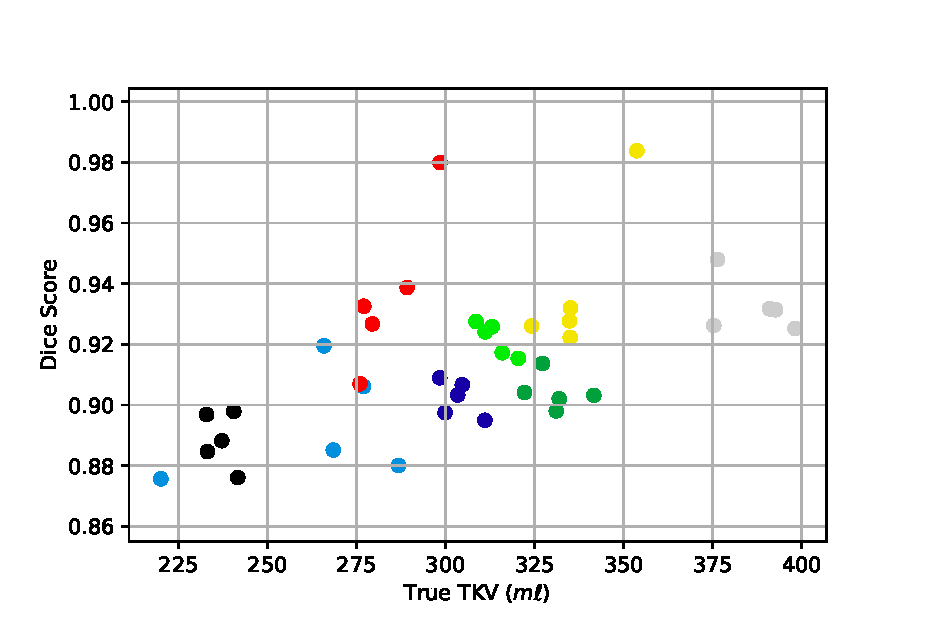
\includegraphics[width=.47\textwidth]{ML/BA_plots/190802_training_data_shuffle_input_and_slices_max_dice_09013_validation_dice.eps}
	\caption{The dice scores for all volumes in the validation data. Each subject is plot in a different colour.}
	\label{fig:ml_validation_dice}
\end{figure}

The mean dice score over all forty volumes is 0.91$\pm$0.02. Here we see a slight trend towards more accurate predictions for larger kidneys. The reason for this becomes clear when we look at the \ac{ROI} the algorithm is outputting, Figure \ref{fig:ml_roi}.

\begin{figure}[H]
	\centering
	\begin{subfigure}[c]{0.47\textwidth}
		\centering
		\includegraphics[width=1\textwidth]{ML/ROI/Kidney_vols2_repro3_T2W_TSE_Cor_BH_60_2_1_sl_01.png}
		\caption{}
		\label{fig:ml_roi_outside}
	\end{subfigure}
	\hfill
	\begin{subfigure}[c]{0.47\textwidth}
		\centering
		\includegraphics[width=1\textwidth]{ML/ROI/Kidney_vols2_repro3_T2W_TSE_Cor_BH_60_2_1_sl_08.png}
		\caption{}
		\label{fig:ml_roi_inside}
	\end{subfigure}
	\caption{(\subref{fig:ml_roi_outside}) A slice from the posterior of the volume. (\subref{fig:ml_roi_inside}) A slice from the centre of the kidneys.}
	\label{fig:ml_roi}
\end{figure}

In Figure \ref{fig:ml_roi_outside} the algorithm is assigning false positives on the right hand side of the image in the area a kidney would be expected further into the body. The amount of false positives decrease as the slices move in an anterior direction as kidney comes into the slice, \ref{fig:ml_roi_inside}. The algorithm works on each slice individually as a two-dimensional image rather than as a three-dimensional volume. This means that, as the majority of slices in the training data have two kidneys in them, the algorithm is more likely to generate false positives if there is no kidney in the slice. For smaller kidneys, there are more slices with no kidney in them and therefore the overall dice score is lower, hence the trend observed in Figure \ref{fig:ml_validation_dice}.

There are multiple methods of reducing this tendency in the algorithm. The false positives tend to be spatially independent through slices, this means that it would be relatively simple to remove them in post-processing by reconstructing the two-dimensional slices back into a three-dimensional volume and removing masked areas with a small volume or areas that are very thin in the anterior-posterior direction. Another method would be to modify the architecture to a \ac{RNN} with \ac{LSTM}. This would also keep the large advantage of working with two-dimensional images, that the algorithm generalises to $n$ slices, but means that the algorithm also has some memory of what is in the surrounding slices \cite{chen_combining_2016, stollenga_parallel_2015}. Finally the algorithm could be re-written as a three-dimensional \ac{FCN}, this would give the greatest degree of accuracy between slices however comes at the expense of simple generalisation with regards to number of slices or the slice thickness and would require much more data collection as amount of training/test data would be reduced by a factor of approximately thirteen.

To establish how the network is performing with the relatively small amount of training data, predictions were made on the training and testing data and the dice score plot, Figure \ref{fig:ml_training_dice}.

\begin{figure}[H]
	\centering
	\includegraphics[width=.5\textwidth]{ML/BA_plots/190802_training_data_shuffle_input_and_slices_max_dice_09013_training_dice.eps}
	\caption{The dice score of predictions made on the training data.}
	\label{fig:ml_training_dice}
\end{figure}

The algorithm is performing better on most of the training data than it did on the validation data although with 80\% of the volumes segmented more accurately than the validation data. This indicates that a certain degree of over fitting is occurring as the 20\% of volumes that are not segmented as well are most likely the testing data. Earlier in the development of this network it was established that augmentation did not improve the performance of the trained network however this should be explored again in light of this result as some basic augmentation would lead to a smaller disparity between the training data and test data and thus allow for better performance when segmenting the validation data.

An indication that some degree of data augmentation would be beneficial is also seen when investigating if there is any difference in performance of the network between healthy and \ac{CKD} kidneys. The manually segmented mean \ac{TKV} of the healthy subjects is 330$\pm$35 m$\ell$ and for subjects with \ac{CKD} is 268$\pm$32 m$\ell$ therefore it would be expected that the algorithm would perform better on the healthy subjects given their larger kidney volume. This is not the case though, the mean dice score of the validation images for healthy kidneys is 0.89$\pm$0.02 and for kidneys with \ac{CKD} this increases to 0.93$\pm$0.02. As there are more healthy subjects in the training data (26 versus 23) it would be expected that the network would perform better for these subjects however the greater degree of variability in geometry and size of the \ac{CKD} kidneys means they essentially have some degree of augmentation built into them. If this were replicated via data augmentation in the whole training dataset then an increase in accuracy across the board may be observed.

\newpage
\section{Conclusions and Future Work}

This method has been shown to produce promising results delivering an mean dice score of 0.91$\pm$0.02 over eight unseen scans with a mixture of healthy and \ac{CKD} subjects resulting in a mean \ac{TKV} difference of 0.69\% when compared to the manually segmented \ac{TKV}. This is especially promising as the algorithm will improve in accuracy as more training data is collected, something which the renal group at \ac{SPMIC} are actively pursuing by adding this scan to almost every subject that goes in the scanner. Efforts have been made to avoid the quintessential machine learning mistakes such as imbalanced training data making the algorithm too specific and un-generalisable and the network only working for healthy subjects. We have also peaked inside the black box of the algorithm to check that it is behaving in a sensible and expected manner.

There is still work to be done on this segmentation method, as explained above, there are signs that data augmentation may improve both the accuracy and generalisability of the algorithm, this should be implemented and evaluated. By implementing data augmentation, the false positives observed on fringe slices may decrease however, if this is not the case then there are multiple solutions to reduce the prevalence of these errors such as basic binary filtering or modifying the networks architecture. There seems to be a reasonable degree of variability in the manually segmented data, to investigate this, the manual masking process should be repeated by a second observer at assess if this variability in the data is due to acquisition or human interpretation.

Another common segmentation task in renal imaging is to generate \ac{ROI} for the renal cortex and medulla. There are some automated methods of achieving this once an overall renal mask has been produced \cite{cox_multiparametric_2017}, however there has been no work on the application of machine learning to this task. During the acquisition of the $T_2$ weighted data in Section \ref{sec:ml_methods_acquisition}, a sequence designed to optimise the contrast between cortex and medulla was also collected on each subject, an example of which is shown in Figure \ref{fig:ml_t1}. Using this data it may be possible to develop the algorithm further so it can segment each tissue type within the kidneys.

\begin{figure}[H]
	\centering
	\includegraphics[width=.4\textwidth]{ML/T1/T1W.png}
	\caption{An example of the data collected to enable segmentation of the renal cortex and medulla.}
	\label{fig:ml_t1}
\end{figure}

Ultimately the goal of this work is to produce an easy to use segmentation tool that can be utilised by clinicians and scientists alike. As such, time should be spent making the software easy to use with a simple front end/\ac{GUI}.

\section{Acknowledgements}

We gratefully acknowledge the support of NVIDIA Corporation with the donation of the Titan Xp GPU used for this research.

\newpage
\section{References}
\defbibheading{bibliography}[\refname]{}
\printbibliography